\chapter{Marco Teórico} \label{chap:marcoteorico}

En el siguiente capitulo se pondrá al alcance del lector las bases teóricas y los conocimientos necesarios para poder entender las diferentes terminologías utilizadas en este trabajo de investigación realizado.

Se tratará de dar un enfoque simplificado de temas como: ¿que es el sensado remoto?, ¿que es Machine Learning y Computer Vision?, un breve repaso de modelos de optimización, cuales son las técnicas y modelos utilizado de validación para el cálculo de métricas. 
Por ultimo se describirá los tipos de clasificadores que existen en la actualidad.

\section{Sensado Remoto}\label{sec:sensadoremoto}

Para comenzar vamos a hablar del principal enfoque de este trabajo que son las imágenes satelitales. Comenzaremos desarrollando desde como formamos una imagen satelital, cuales son los rango de bandas, que instrumento se utiliza y los datos en el cual se trabaja.

\subsection{Teledetección}\label{sub:teledeteccion}

Para comenzar a introducir el concepto de imagen satelital debemos saber como esta formada la misma, es por esto que vamos a desarrollar el concepto de \textit{teledetección}.

La teledetección o sensado remoto también llamado es el proceso que nos permite obtener una imagen de la superficie terrestre de forma remota, es decir sin estar en contacto con ella. Una imagen satelital es una representación de estos datos reflejados por la superficie terrestre que son captadas por un sensor que se encuentran a bordo de un satélite artificial (ver fig \ref{Fig:teledeteccion}).

La teledetección no es mas que la detección de propiedades relevantes del entorno; esta capacidad no es despreciable, nos permite desarrollar aplicaciones practicas con un impacto cada ves mayor \citep{percepcion}. 

En general la teledetección es la medición de energía emanada de la superficie terrestre. Existen diferentes fuentes de energía; si la fuente de energía es el sol entonces lo llamamos \textit{teledetección pasiva}, si la energía medida no es emitida por el Sol, es decir es emitida por un sensor, llamamos \textit{teledetección activa}, como por ejemplo los sensores de radar que funcionan en el rango de microondas.

Los componentes básicos de un sistema de teledetección incluye lo siguiente \citep{chuvieco}:
\begin{itemize}
\item \textit{Fuente de energía}: es la radiación electromagnética que capta el sensor; como mencionamos anteriormente puede tratarse de una fuente pasiva o activa.

\item \textit{Cubierta terrestre}: rasgos naturales o realizados por el hombre, ejemplo construcciones, que refleja el sensor.

\item \textit{Sistema Sensor}: esta compuesto por, cámaras, radar, etc; y la plataforma en la que esta puesto (satélite, avión, globo);  capta la energía proveniente de la tierra y la almacena o envía al sistema de recepción.

\item \textit{Sistema de Recepción}: sistema encargado de recibir la información proveniente del sensor y almacenar en un formato apropiado para luego ser distribuido a los usuarios.

\item \textit{Interprete}: encargado de manipular los datos de acuerdo a la temática de interés (agricultura, catastro, etc), es decir aplica diferentes niveles de procesamiento sobre los datos crudos obtenidos por el sensor.

\item \textit{Usuario Final}: es el consumidor final de la imagen adquirida.
\end{itemize}

\begin{figure}[H] \centering
  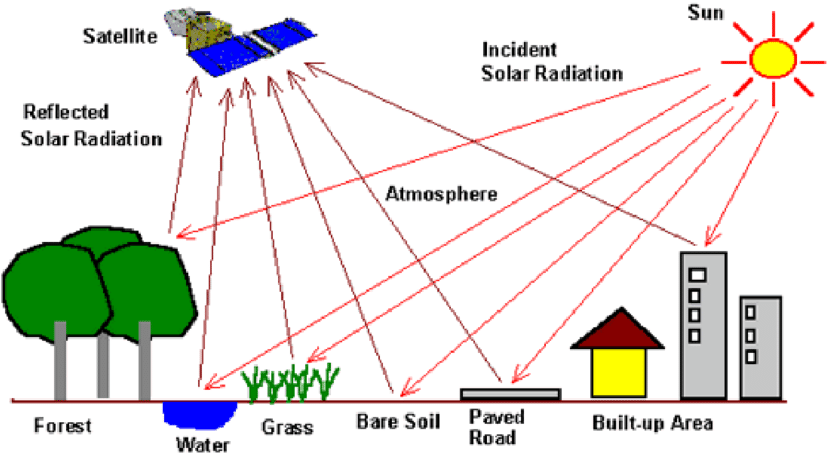
\includegraphics[height=8cm,keepaspectratio=true,clip=true]{imagenes/MarcoTeorico/teledeteccion.png}
  \caption{Sensado Remoto. Navarrete, Edison, Laubacher, Gerard}\label{Fig:teledeteccion}
\end{figure}

\subsubsection{Tipos de Sensores}
\begin{itemize}
\item \textbf{sensores pasivos}: son aquellos que reciben las señales emitidas naturalmente que fueron reflejadas por los objetos. Estas señales son a partir de la radiación solar natural. Este tipo de sensores son  usados mayormente en aplicaciones de evaluación de recursos naturales. Ejemplo: ASTER, MODIS, VIIRS, LandSat.

\item \textbf{sensores activos}: son aquellos que emiten radiación dirigida hacia un objetivo especifico, esta radiación reflejada del objeto es detectada y medida por el sensor. Ejemplo: Radar, Sonar.
\end{itemize}

\subsubsection{Espectro electromagnético}

El espectro electromagnético se denomina al conjunto de todas las longitudes de onda \citep{chuvieco}. Las ondas electromagnéticas cubren una amplia gama de frecuencias o de longitudes de ondas y pueden clasificarse según su principal fuente de producción. 
Las regiones utilizadas para la observación remota de la tierra son:
\begin{itemize}
\item Espectro visible (0.4 - 0.7 µm): rango de frecuencias del ojo humano; máxima radiación solar. Subdividido en tres bandas: Rojo (0.6 - 0.7 µm), Verde (0.5 - 0.6 µm) y Azul (0.4 - 0.5 µm).

\item Infrarrojo cercano (0.7 - 1.1 µm): denominado IR fotográfico o reflejado; energía solar que reflejan los cuerpos. Comportamiento similar al espectro visible.

\item Infrarrojo medio (1.1 – 8 µm): se entremezclan radiación solar y emisión; la atmósfera afecta sensiblemente: aprovechado para medir concentraciones de vapor de agua, ozono, aerosoles, etc.

\item Infrarrojo térmico (8 - 14 µm): radiaciones emitidas por los propios cuerpos; se puede determinar la Temperatura de un cuerpo (IRtérmico). Se puede disponer de imágenes a cualquier hora del día.

\item Microondas (1mm-1m): Interés creciente de la Teledetección en esta banda; las perturbaciones atmosféricas son menores y es transparente a las nubes. Se suelen utilizar sensores activos. 

\end{itemize}

\begin{figure}[H] \centering
  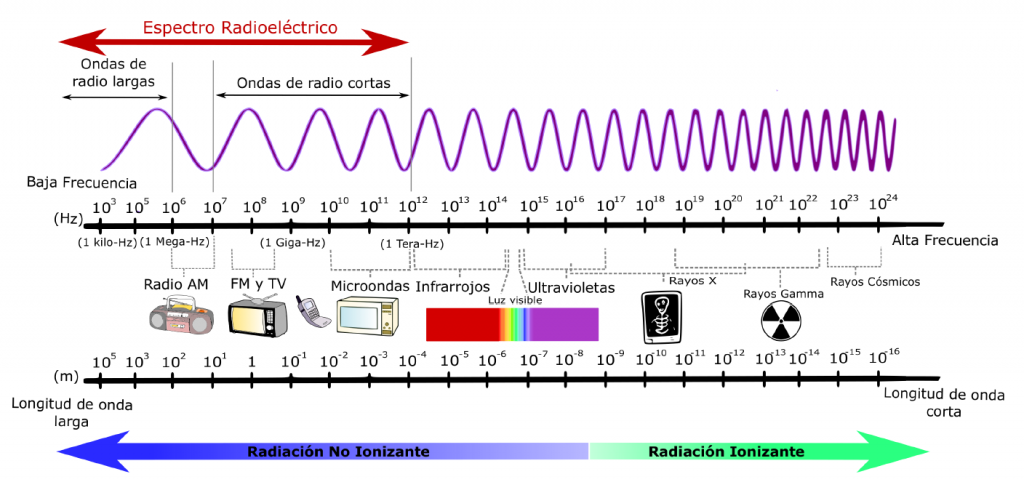
\includegraphics[height=8cm,keepaspectratio=true,clip=true]{imagenes/MarcoTeorico/espectro-electro.png}
  \caption{Espectro electromagnético}\label{Fig:espectro-electromagnetico}
\end{figure}


\subsubsection{Resolución}
Unas de las características de los sensores son el tipo de imagen que proporciona; estas características vienen definidas por el timpo de resolución. Estas resoluciones la podemos definir de la siguiente manera:

\begin{itemize}
\item \textbf{Resolución Espacial}: distancia que corresponde a la unidad mínima de información incluida en un píxel. A menor tamaño de píxel mayor sera la resolución espacial, esto quiere decir que el sensor tendrá mayor detalle de los objetos.

\begin{figure}[H] \centering
  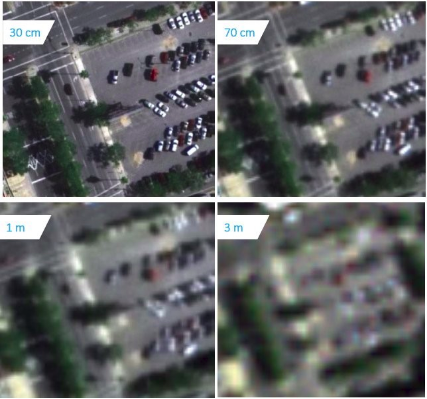
\includegraphics[height=8cm,keepaspectratio=true,clip=true]{imagenes/MarcoTeorico/resolucion.png}
  \caption[Resolución espacial]{Resolución espacial\footnote{//iie.fing.edu.uy/proyectos/esopo/eem/}} \label{Fig:resolucion-esp}
\end{figure}

\item \textbf{Resolución Espectral}: la resolución espectral especifica el numero y la anchura de las badas espectrales que puede ser discrimidadas por el sensor.
\begin{figure}[H] \centering
  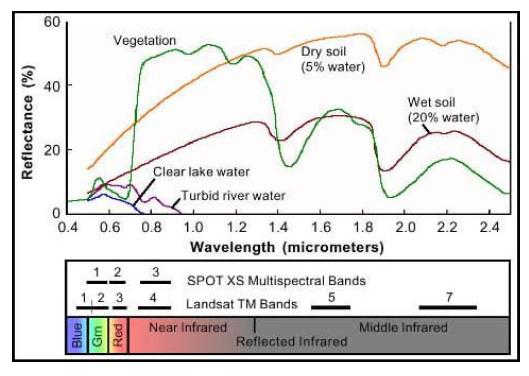
\includegraphics[height=8cm,keepaspectratio=true,clip=true]{imagenes/MarcoTeorico/resolucion_espectral.jpg}
  \caption[Resolución espectral]{Resolución espectral\footnote{http://laotraopinion.net/wp-content/uploads/poder-de-resolucion-espectral.jpg}}\label{Fig:resolucion-espectral}
\end{figure}

\item \textbf{Resolución Radiometrica}: indica el numero de bits utilizados para expresar los datos recogidos por el sensor. Mayormente cuando es mas grande el número de niveles mayor es el detalle con la cual se podrá expresar dicha información. Ejemplo los sensores Landsat (5 y 7) utilizan 8 bits lo que da 2**8= 256 niveles de energía que pueden ser captados.
\begin{figure}[H] \centering
  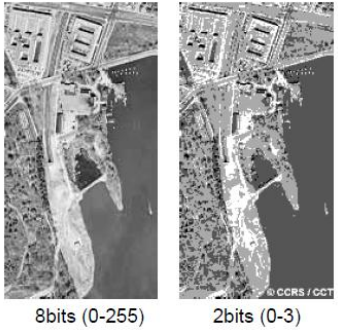
\includegraphics[height=8cm,keepaspectratio=true,clip=true]{imagenes/MarcoTeorico/resolucion_radiometrica.png}
  \caption{Resolución radiometrica}\label{Fig:resolucion-radiometrica}
\end{figure}

\item \textbf{Resolución temporal}: es el tiempo necesario que tarda el satélite en volver a visitar la misma zona de la Tierra; es decir la periodicidad con la que éste adquiere la misma imagen. Este ciclo de cobertura esta en función de el tipo de orbita de la plataforma así como del sensor. Alta resolución temporal (< 1 día - 3 días), media resolución temporal (4 - 16 días), baja resolución temporal (> 16 días).

\end{itemize}

\subsubsection{Imagen Satelital}

Una imagen satelital esta compuesta por diferentes matrices de las cuales cada celda representa un píxel; la dimensiones de depende del tipo de resolución espacial como se mencionó anteriormente. Los sensores almacenan la radiación electromagnética proveniente de distintas coberturas y las almacena en el píxel de acuerdo a los intervalos de onda correspondiente de cada sensor. Esta energía electromagnética se representa en cada píxel por un valor digital llamado Nivel Digital (ND), la cantidad de ND que se podrá representar depende de la resolución radiométrica.

La asignación de colores más conocido por los usuarios es el \textit{falso color} (R=Red (rojo); G=Green (verde); B=Blue (azul)), la cual asigna el color azul a la banda del verde, el color verde a la banda del rojo y el color rojo a la banda del infrarrojo cercano. La información obtenida de diferentes combinaciones de bandas depende del objeto de estudio que se esta llevando a cabo.

%https://acolita.com/wp-content/uploads/2018/01/Teledeteccion_espacial_ArcGeek.pdf
%https://mundosigs.wordpress.com/2016/03/07/que-son-los-sensores-remotos/
%https://www.slideshare.net/noldinn/fundamentos-deteledeteccionemiliochuvieco

\section{Aprendizaje Automático}

\subsection{Machine Learning}
\ac{ml} como se mencionó en la primera sección, es una rama de la inteligencia artificial que tiene como objetivo desarrollar técnicas que ayuden a las computadoras a aprender determinado comportamiento, generalizando, a partir de los datos de entrada. Un algoritmo de \ac{ml} es aquel que permite aprender a partir del conjunto de datos. \ac{ml} nos permite abordar tareas que son muy difíciles de resolver con programas escritos y diseñados por seres humanos.

"Se dice que un programa de computadora aprende de la experiencia E con respecto a algún tipo de tareas T y la medida de rendimiento P, si su desempeño en tareas en T, medido por P, mejora con la experiencia E." \citep{Mitchell}

Existen una gran cantidad de problemas que caen dentro de este tipo de rama, que podemos nombrar a continuación:

\begin{itemize}
\item \textit{Problemas de Regresión}: Este tipo de problema se pide que la computadora prediga un valor numérico dada alguna entrada. Los ejemplos que podemos citar son: fijar el precio de una casa a partir de las característica de la misma (cantidad de habitaciones, baños, etc), predecir el valor de la bolsa a partir del comportamiento de la bolsa en el tiempo pasado, entre otros.

\begin{figure}[H] \centering
  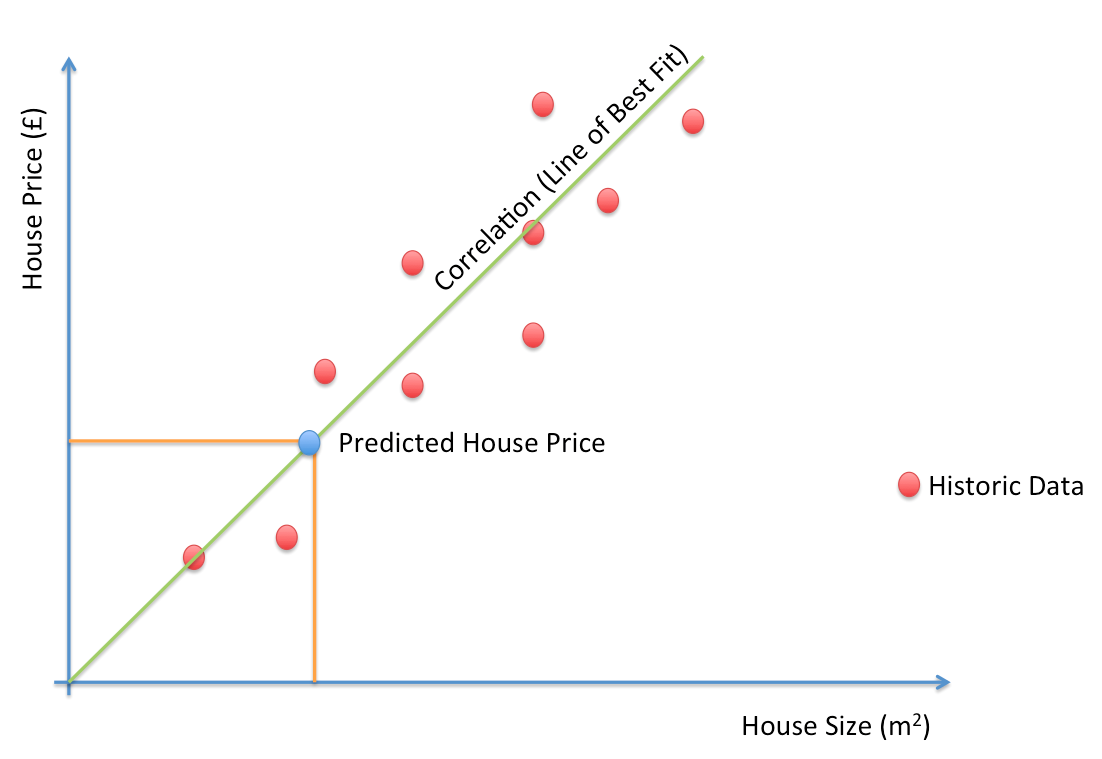
\includegraphics[height=8cm,keepaspectratio=true,clip=true]{imagenes/MarcoTeorico/regression_linear.png}
  \caption{Ejemplo Regresión (precio de una casa)}\label{Fig:regression}
\end{figure}

\item \textit{Problemas de Clasificación}: En un problema de clasificación, estamos tratando de predecir los resultados en una
salida discreta. En otras palabras, estamos tratando de asignar variables de entrada en categorías discretas. Algunos de los ejemplos son: clasificar perros o gatos determinando a que clase pertenece la imagen, evaluar si un e-mail pertenece a la categoría "spam" o "no spam", entre otros.

\begin{figure}[H] \centering
  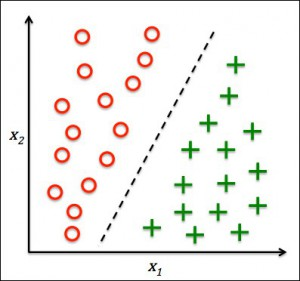
\includegraphics[height=8cm,keepaspectratio=true,clip=true]{imagenes/MarcoTeorico/classification.jpg}
  \caption{Ejemplo Clasificación}\label{Fig:clasificacion}
\end{figure}


\item \textit{Problemas de Aprendizaje no supervisado}: El aprendizaje no supervisado nos permite abordar los problemas con
poca o ninguna idea de cómo deben ser nuestros resultados. Podemos derivar la estructura de los datos donde no necesariamente conocemos el efecto de las variables. Podemos derivar esta estructura agrupando los datos basados en relaciones entre las variables en los datos. Con el aprendizaje no supervisado no hay una retroalimentación basada en los resultados de la predicción. El objetivo de problemas de aprendizaje no supervisados puede ser descubrir grupos de ejemplos similares dentro de los datos, donde se denomina agrupación (clustering), o determinar la distribución de datos dentro del espacio de entrada, conocida como estimación de densidad (density estimación), o proyectar los datos desde un espacio de nivel dimensional alto hasta dos o tres dimensiones con propósitos de visualización \citep{bishop}.

\begin{figure}[H] \centering
  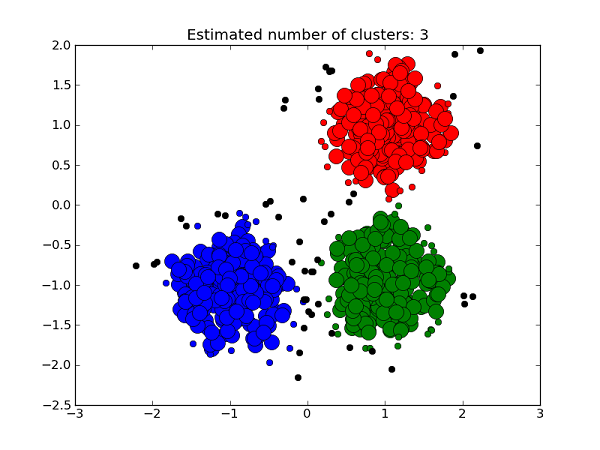
\includegraphics[height=8cm,keepaspectratio=true,clip=true]{imagenes/MarcoTeorico/claustering.png}
  \caption{Ejemplo aprendizaje no supervisado, claustering}\label{Fig:clauster}
\end{figure}
\end{itemize}

\subsubsection{Entrenamiento del modelo}
%https://docs.aws.amazon.com/es_es/machine-learning/latest/dg/training-ml-models.html
%clasificación supervisada metodos deduccion matematica
Entrenar un modelo de \ac{ml} consiste en proporcionar un conjunto de datos de entradas, datos de entrenamiento, de las cuales el algoritmo va a aprender. El algoritmo encuentra patrones en los datos proporcionados de entrada y genera un modelo que captura y generaliza dichos patrones para luego realizar predicciones sobre datos que no conoce.

Para poder entrenar un modelo necesitamos al menos tres cosas especificas:
\begin{enumerate}
\item \textbf{Datos de entrada}: determinar cuales son los ejemplos de entrada del algoritmo; el objetivo es crear un modelo que generalice los nuevos datos, para esto los datos de entrada deben ser representativo del mundo real. Por ejemplo para una tarea de clasificación entre perros y gatos los datos de entrada deben ser imágenes que pertenezcan a las categorías mencionadas; para resolver un problema de reconocimiento de voz los datos de entrada deben ser audios de personas hablando.

\item \textbf{Salida esperada}: para cada valor de entrada debemos etiquetar a que clase pertenece es decir, para un problema de clasificación entre perros y gatos debemos tener etiquetada cada imagen para saber a que clase pertenece la imagen; para un ejemplo de reconocimiento de voz cada audio debe tener una transcripción del mismo.

\item \textbf{Evaluación de las predicciones}: calcular y evaluar métricas con los resultados de la predicciones obtenidas por los modelo, es decir, determinar la distancia entre la salida esperada y los valores predichos.
\end{enumerate}

Como se desarrollo anteriormente el proceso de entrenamiento tiene: variables de entrada (x) y una variable de salida (Y); que a través de un algoritmo de aprendizaje obtenemos la siguiente relación entre estas variables como vemos a continuación.


\begin{eqnarray}
 f:X \longrightarrow Y\\
 \mbox{Training}:\qquad \{(x^i, y^i) \in X\; x\; Y \} _i=1...n\\
 \mbox{El objetivo es encontrar}\; f\; \mbox{tal que:}\qquad f(x)\approx y
\end{eqnarray}

Considerando el siguiente ejemplo, dada las coordenadas (x,y) como se muestra en la siguiente figura \ref{Fig:ejemplo-1}, se muestran dos clases, puntos de color negro y otra blanca.
\begin{figure}[H] \centering
  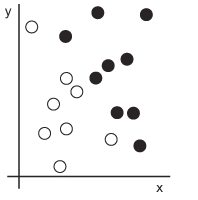
\includegraphics[height=4cm,keepaspectratio=true,clip=true]{imagenes/MarcoTeorico/sample.png}
  \caption{Ejemplo entrenamiento}\label{Fig:ejemplo-1}
\end{figure}

La idea principal de desarrollar un modelo; es crear un algoritmo que a partir de datos encuentre automáticamente una frontera, clasifique, encuentre por ejemplo una frontera entre los puntos negros y los puntos blancos.

Como se puede ver en la figura siguiente \ref{Fig:ejemplo-2}, se muestra la frontera de separación creada por el algoritmo entrenado.
\begin{figure}[H] \centering
  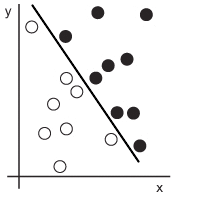
\includegraphics[height=4cm,keepaspectratio=true,clip=true]{imagenes/MarcoTeorico/sample-fit-1.png}
  \caption{Entrenamiento}\label{Fig:ejemplo-2}
\end{figure}

De esta manera cuando se pase un elemento que nunca vio puede determinar en cual de los dos espacios creado por el modelo cae este nuevo dato; en este caso estamos hablando en un algoritmo de clasificación.

\subsubsection*{Ejemplo: Regresión Lineal}
%http://www.deeplearningbook.org/contents/ml.html
Una Regresión lineal es un claro ejemplo de un algoritmo de \ac{ml}; el objetivo es desarrollar un sistema que tome un vector $x \in \; $R$^n$, prediga el valor de un escalar $y \in \; $R$ $ como salida; la salida de una regresión lineal es una función lineal de la entrada.  Vamos a tomar como $\hat{y}$ el valor que nuestro modelo predice definido por:
\begin{equation}
\hat{y} = w^t * x
\end{equation}
donde $w \in \; $R$ $, siendo un vector de parámetros.
Los parámetros son valores que controlan el comportamiento del sistema,en este caso w  multiplicado por x (característica de cada datos de entrada), lo podemos ver como un conjunto de pesos que determinan como cada característica afecta a la predicción.

Si x esta multiplicado por un peso $w_i $ positivo, entonces el valor de esa característica aumenta nuestra predicción, de manera análoga si el valor $w_i $ es negativo esa característica x disminuye mi valor de predicción $\hat{y}$.
Como siguiente medida debemos medir la precisión de nuestro modelo, para realizar la medición de nuestro modelo debemos anteriormente haber separado el conjunto de datos en dos partes por un lado los datos de que se van a usar para realizar el entrenamiento y por otro los datos que serán utilizados para medir la precisión del modelo, llamado conjunto de test.

Una de las maneras de medir nuestra precisión del modelo con nuestro conjunto de test es computando el error cuadrado medio, dado por la siguiente ecuación:
\begin{equation}\label{eqn:mse} 
MSE_{test} = \frac{1}{n}\sum_{i}(\hat{y}^{test}- y^{test})^2
\end{equation}

Como se puede ver a partir del calculo anterior el error decremento a 0 cuando $\hat{y}$ es igual a $y$. Para entrenar un modelo de \ac{ml} necesitamos realizar un algoritmo que en cada iteración mejore los valores de los pesos de manera de reducir el error; en la sección siguiente se desarrollará mas en detalle.

Decimos que una hipótesis generaliza bien, cuando predice correctamente con entradas no conocidas.

\subsubsection{Función de Costo}
Existen diferentes maneras de que una algoritmo aprenda los parámetros de un modelo, este proceso de aprendizaje es posible minimizando la función de costo. Una función de costo es una medida del cuán erróneo es el modelo que estamos entrenando en términos a la capacidad de estimar la relación entre $X $ e $y $. Esto se lo puede expresar como la diferencia o distancia entre el valor predicho y el actual valor.

Como se menciono anteriormente el objetivo de un modelo de \ac{ml} es encontrar los valores que minimicen la función de costo.Una función de costo toma un conjunto de datos y retorna un valor llamado error costo (\textit{loss cost} su traducción en ingles). Existen diferentes tipos de funciones de costo que podemos usar; una de las mas comunes usada es \textbf{mean square error}, MSE, visto en \ref{eqn:mse}, en este caso determina la distancia o simplemente la diferencia entre el dato y el predictor $(x_i - y_i) $ ver figura: \ref{Fig:mse}.
\begin{figure}[H] \centering
  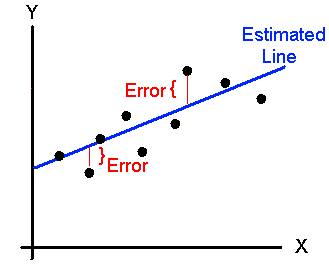
\includegraphics[height=4cm,keepaspectratio=true,clip=true]{imagenes/MarcoTeorico/mse-cost.png}
  \caption{Mean Square Error }\label{Fig:mse}
  %http://wiki.fast.ai/images/5/55/Linear_line_w_cost_function.png
\end{figure}

Dado un punto de datos $(x_i,y_i) $, donde $x_i $ es el conjunto de característica (por ejemplo pisos, dormitorios, etc) que el modelo usa para realizar la predicción, $y_i $ es la etiqueta del ejemplo (por ejemplo precio de la casa) e $y(x_i)$ es la la función de predicción; el error esta dado por la siguiente formula:
\begin{equation}\label{eqn:error-mse}
e = (y(x_i) - y_i)^2
\end{equation} 
A partir del calculo anterior podemos generalizar y tomar el promedio sobre todo los punto de datos de la siguiente manera:
\begin{equation}
MSE =  \frac{1}{n}\sum_{i}(y_i - y(x_i))^2
\end{equation}
% NOTA: SE DEBE PONER MAS FUNCIONES DE COSTO RMSE?

Existen en la actualidad diversas funciones de costo que nos permite calcular el error del modelo; entre ellas están: Quadratic cost, Cross-entropy cost, Exponentional cost, Hellinger distance, Kullback–Leibler divergence, entre otras.

%https://stats.stackexchange.com/questions/154879/a-list-of-cost-functions-used-in-neural-networks-alongside-applications

\subsubsection{Algoritmos de Optimización} 
%https://hackernoon.com/gradient-descent-aynk-7cbe95a778da
%https://stxlearning.com/2018/03/25/optimizacion-deep-learning-y-complejidad-computacional/
En modelos de \ac{ml} debemos encontrar aquellos parámetros que minimizan la función de costo como se menciono previamente, este es un problema de optimización ya que si encontramos la solución podemos encontrar esos parámetros que disminuyen el error.

En la mayoría de los algoritmos de \ac{ml} deben aprender mas de un parámetro, en algunos casos hasta decenas de millones de parámetros; es por esto que todos los algoritmos  son métodos de optimización ya que se busca aprender los parámetros de manera eficiente. La estrategia mas típica para problemas de optimización son los llamados métodos de descenso; dentro de estos se encuentran: descenso de gradiente, descenso de gradiente estocástico y método de Newton Rawson de 2 orden.

\subsubsection*{Descenso de gradiente}\label{sub:gradient-desc}
Para encontrar el mínimo valor para grandes dimensiones de datos el algoritmo mas utilizado es el llamado \textbf{Descenso de Gradiente} (\textit{gradient descent} en ingles). El descenso de gradiente es un algoritmo de optimización que busca encontrar el mínimo local o global de una función convexa.  En \ac{ml} usamos descenso de gradiente para encontrar los parámetros de nuestro modelo que mejor definen nuestro conjunto de entrenamiento.

Este algoritmo permite que el modelo aprenda el gradiente o la dirección que el modelo debe seguir para reducir el error; en cada iteración gradualmente converge hacia un mínimo optimizando los valores $w_i $ que minimizan la función de costo. $$\min_{w} f(w)$$

Esto quiere decir que queremos encontrar los parámetros $w$ que minimicen la diferencia entre las salidas $Y$ y las producidas por el modelo dependiente de $w$. Entre menor  diferencia mejor aproximación a la salida $Y$. 

\begin{figure}[H] \centering
  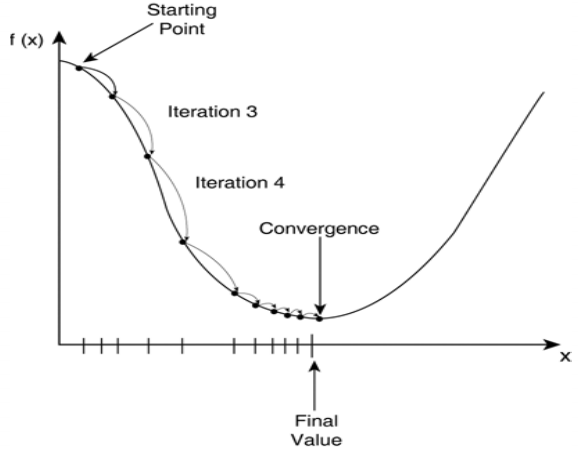
\includegraphics[height=6cm,keepaspectratio=true,clip=true]{imagenes/MarcoTeorico/gradient-descent.png}
  \caption{Gradient Descent }\label{Fig:gradient-descent}
\end{figure}


%Gradiente extraido de :https://www.cs.huji.ac.il/~shais/UnderstandingMachineLearning/understanding-machine-learning-theory-algorithms.pdf
El gradiente de una función diferenciable $ f: R^d \longrightarrow R $ en $\textbf{w}$, denotado $ \nabla f(w) $ vector de derivadas parciales de la función $f$ es decir:
\begin{equation}
\nabla f(x) = (\frac{\partial f(\textbf{w})}{\partial w[1]},....., \frac{\partial f(\textbf{w})}{\partial w[d]})
\end{equation}

Descenso de gradiente es un algoritmo iterativo; comenzamos con un valor inicial de $\textbf{w}$ (el valor 0 por ejemplo), luego en cada iteración damos un paso en la dirección negativa del gradiente en el punto actual. Es decir, el paso de actualización es:
\begin{equation}
\textbf{w}^{(t-1)} = \textbf{w}^{(t)} - n \nabla f(\textbf{w}^{(t)})
\end{equation}
En el cual $n > 0$, dado que el gradiente apunta a la dirección del mayor índice de $f$ alrededor $w^{(t)}$, el algoritmo va en sentido opuesto disminuyendo el valor de la función. Luego de T iteraciones se genera un vector promedio dado por: $ \hat{w} = \frac{1}{T} \sum_{t=1}^T w^{(t)}$; la salida también puede ser el vector con mayor  $ argmin_{t \in [T]} f(w^{(t)}) $.


En dónde $\hat{w}$ es una nueva posición de los parámetros que se acercan más al mínimo buscado, es decir que hacen que $f(w^{(t)})$ aproxime mejor a $Y$ . Existen diversas variantes de descenso por gradiente como Batch gradient descent, Stochastic gradient descent y Mini-batch gradient descent.

% PONEMOS BACKPROPAGATION, LEARNING RATE
%http://ruder.io/optimizing-gradient-descent/
%https://turing.iimas.unam.mx/~ivanvladimir/posts/gradient_descent/

\subsubsection{Validación de Modelos}\label{sub:validacion-modelo}

Antes de evaluar nuestro modelo debemos separar nuestro datos en: \textit{datos de entrenamiento} y \textit{datos de test}; en la mayoría de los casos se suele realizar una separación del conjunto de datos total en porcentajes de 60/40, 70/30 o 80/20 para entrenamiento y test.

Una de las principales causas de validar nuestro modelo son obtener resultados erróneos en la predicción; esta causa esta dada por dos términos muy importante que debemos tener en cuenta: \textbf{overfitting y underfitting}. \textit{\textbf{Overfitting}} y \textit{\textbf{underfitting}} son dos grandes problemas en \ac{ml} que influye en la performance del modelo. 

\subsubsection*{Overfitting}
Este concepto en \ac{ml} hace referencia al sobre-entrenamiento del modelo. El overfitting ocurre cuando un modelo aprende en detalle junto al ruido en los datos de entrenamiento afectando negativamente el rendimiento del modelo en los nuevos datos a predecir. Esto significa que el ruido o las fluctuaciones aleatorias en los datos de entrenamiento son aprendidos como conceptos por el modelo. El problema es que estos conceptos no se aplican a los nuevos datos e impactan negativamente en la capacidad de generalización de los modelos.

\subsubsection*{Underfitting}
Como parte opuesta al overfitting esta el  underfitting; este concepto hace referencia a aquellos modelos que no pueden generalizar nuevos datos de entrenamiento de manera correcta. Mayormente en problemas de underfitting se necesita mayores características de los datos para la construcción de los modelos.

\begin{figure}[h]
 \centering
  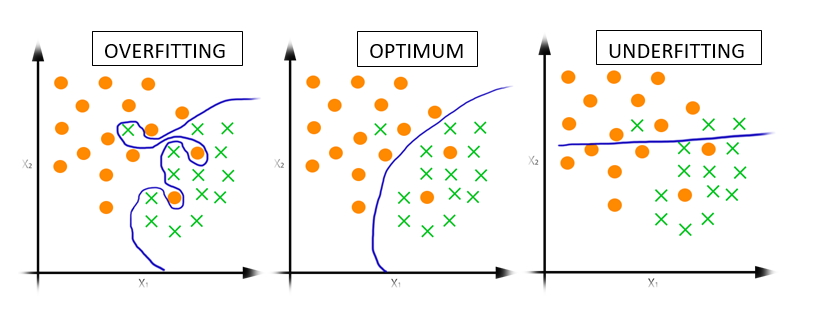
\includegraphics[height=5cm,keepaspectratio=true,clip=true]{imagenes/Logos/OverFUnderF.png}
  \caption{Ejemplo de overfitting (izquierda), modelo óptimo (centro) y underfitting (derecha)}
	\label{Fig: overUnder}
\end{figure}


Existen diferentes técnicas para validar la robustez de nuestro modelo y evitar los problemas mencionados anteriormente, una de ellas es por  \textit{validación cruzada} (cross validation en ingles). La validación cruzada es una técnica que evalúa los resultados de un análisis estadístico y garantiza de que sean independientes de la partición de los datos de entrenamiento y prueba. 

Hay diversos tipos de validación cruzada, de las cuales podemos nombrar:

\begin{enumerate}

\item \textbf{K-Fold Cross Validation}: consiste en dividir el conjunto de datos en \textit{k} subconjuntos. Existe un $k-1 $ valor que es el de validación, es decir, se toma uno de los subconjunto y se los utiliza como validación y el resto como entrenamiento.  Este proceso se repite durante $k $ iteraciones con cada uno de los subconjunto de dato de validación. Para finalizar se utilizar aquel subconjunto de datos que posea mayor generalidad.
\begin{figure}[H]
 \centering
  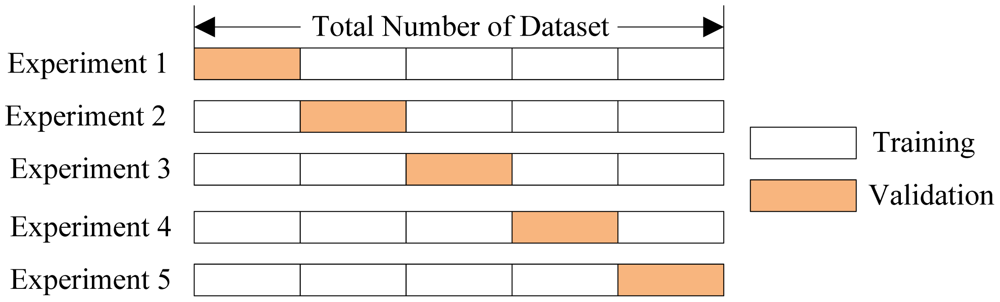
\includegraphics[height=5cm,keepaspectratio=true,clip=true]{imagenes/Logos/crossvalidat.png}
  \caption{Validación cruzada para k=5\\(Adaptado de:{http: //goo.gl/Dp85h3})}
	\label{Fig: crossvalidation}
\end{figure}

\item \textbf{Leave-One-Out Cross-Validation (LOOCV)}: Es un caso particular de validación cruzada, tomamos todos los datos que poseemos y utilizamos solo uno del subconjunto para validar. La ventaja de este método es que usamos todo los datos para realizar el entrenamiento.

\begin{figure}[H]
 \centering
  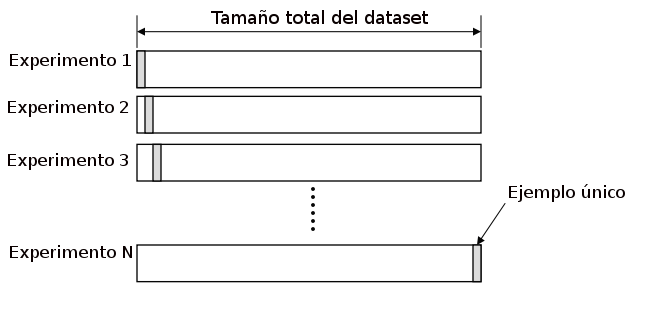
\includegraphics[height=5cm,keepaspectratio=true,clip=true]{imagenes/MarcoTeorico/cross-validation-LOOCV.png}
  \caption{Leave-One-Out Cross-Validation (LOOCV)}
	\label{Fig: crossvalidation-LOOCV}
\end{figure}

\item \textbf{Random Subsampling}: En esta técnica, se eligen aleatoriamente múltiples conjuntos de validación y se combinan para formar un conjunto de datos de prueba. Los datos restantes forman el conjunto de datos de entrenamiento.

\begin{figure}[H]
 \centering
  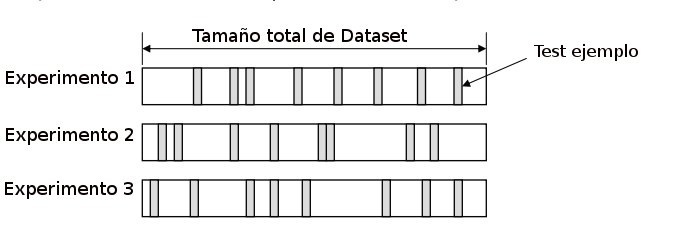
\includegraphics[height=5cm,keepaspectratio=true,clip=true]{imagenes/MarcoTeorico/cross-validation-random.png}
  \caption{Random Subsampling}
	\label{Fig: random-Subsampling}
\end{figure}

\end{enumerate}


%IMPORTANTE: https://sebastianraschka.com/pdf/manuscripts/model-eval.pdf
%https://dzone.com/articles/machine-learning-validation-techniques

\subsubsection{Evaluación de Modelos}\label{sub:evaluación-modelo}
Para determinar la efectividad de un modelo necesitamos realizar un evaluación de cuan bien nuestro modelo puede generalizar los datos y lograr una predicción correcta dado un valor de entrada desconocido. Las técnicas de evaluación en \ac{ml} son usadas para obtener esa tasa de error en el modelo. La forma de validar modelos en \ac{ml} es a través de métricas, la elección de la métrica depende de cada tarea a realizar, es importante revisar este conjunto de métricas para tener la certeza de que nuestro modelo tiene un buen rendimiento. 

El trabajo realizado en esta tesis es un problema de clasificación, es por esto que desarrollaremos las métricas existentes para problemas de clasificación:

\begin{enumerate}
\item \textbf{Matriz de Confusión}, \textit{Confussion Matrix}: contiene información sobre clasificaciones realizadas por el predictor y las etiquetadas, el rendimiento  se evalúa comúnmente utilizando los datos de la matriz.

\begin{figure}[H]
 \centering
  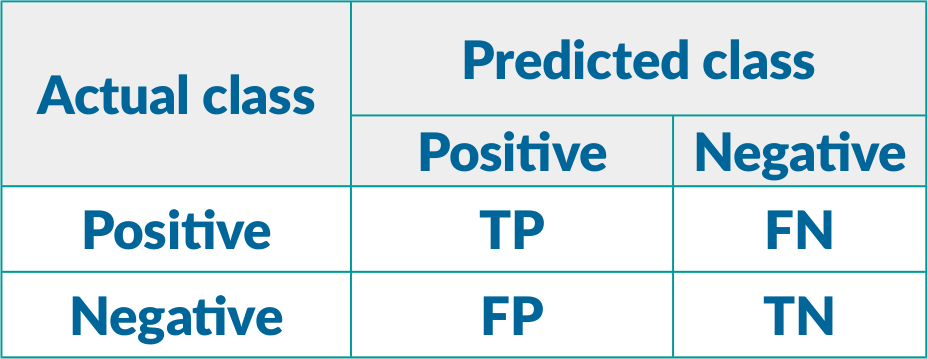
\includegraphics[height=5cm,keepaspectratio=true,clip=true]{imagenes/MarcoTeorico/confussion_matrix.png}
  \caption{Matriz de Confusión}
	\label{Fig: confusion-matrix}
\end{figure}

\begin{itemize}
	\item Positivos (P): Observación positiva (valor etiquetado).
	\item Verdadero Positivo (TP): La observación es positiva y la predicción también.
	\item Falso Negativo (FN): La observación es positiva pero la predicción es negativa.
	\item Falso Positivo (FP): La observación es negativa pero la predicción es positiva.
	\item Verdadero Negativo (TN) :  La observación es negativa y también la predicción negativa.

\end{itemize}


\item \textbf{Accuracy}: Proporción de todas las predicciones que son correctas, da una medida de que tan bueno es el modelo.
\begin{equation}
accuracy = \frac{FP+FN}{FP+FN+TP+TN}=\frac{predicciones\;correctas}{todas\;las\;predicciones}
\end{equation}

\item \textbf{Precisión}: Proporción de todas las predicciones positivas que son correctas. La precisión es una medida de cuántas predicciones positivas son reales.
\begin{equation}
precision=\frac{TP}{TP+FP}= \frac{predicciones\;correctamente\;positivas}{todas\;las\;predicciones\;positivas}
\end{equation}

\item \textbf{Recall}: Nos da la proporción de la observaciones reales positivas que son correcta, es decir nos da la precisión de cuantas observaciones positivas reales se obtuvo correctamente.
\begin{equation}
recall = \frac{TP}{TP+FN} = \frac{TP}{P} = \frac{predicciones\;a\;ser\;positiva}{todas\;la\;observaciones\;positivas} 
\end{equation}

\item \textbf{Overlapping Mean}: Métrica obtenida a partir de la intersección del ground truth y el bounding box de la predicción obtenida \ref{Fig: roc}.

\item \textbf{Curvas ROC}: Representa la capacidad de un modelo para discriminar entre clases positivas y negativas. Un área de 1.0 representa un modelo que hizo perfectamente todas las predicciones.
\begin{figure}[H]
 \centering
  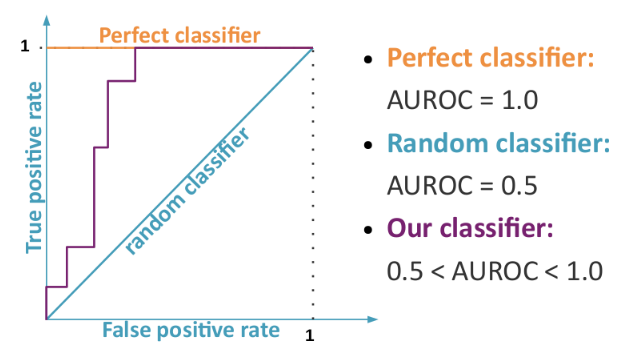
\includegraphics[height=5cm,keepaspectratio=true,clip=true]{imagenes/MarcoTeorico/curvas-roc.png}
  \caption{Curva ROC}
	\label{Fig: roc}
\end{figure}


\end{enumerate}


\subsection{Computer Vision}\label{sub:compueter-vision}
Visión artificial,\ac{cv} por sus siglas en ingles, son aquellas herramientas desarrolladas para extraer información a partir de imágenes.
\begin{figure}[H]
 \centering
  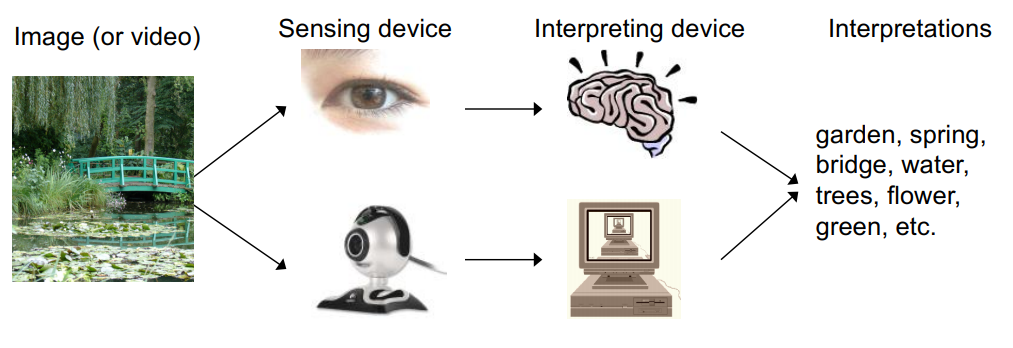
\includegraphics[height=5cm,keepaspectratio=true,clip=true]{imagenes/MarcoTeorico/computer-vision.png}
  \caption{Que es \ac{cv}?, extraido de :(http://vision.stanford.edu)}
	\label{Fig: computer-vision}
\end{figure}

Esta disciplina estudia problemas metodológicos y algorítmicos como así también temas relacionados con la implementación y diseño de soluciones. En los años recientes se convirtió en una tecnología clave en muchos campos debido al gran avance en cámara y en procesamiento computacional.

Un sistema de \ac{cv} actúa sobre una representación de una realidad que le proporciona información sobre brillo colores, formas, etcétera. Estas representaciones suelen estar en forma de imágenes estáticas, escenas tridimensionales o imágenes en movimiento \citep{Ledda}. 


Los campos de aplicación que aplican técnicas de \ac{cv} son en diferentes áreas de la ciencia y la industria \citep{areascv} :
\begin{enumerate}
\item Robótica : Se usan técnicas de \ac{cv} con el fin de reconstruir la escena e identificar los objetos.
\item Biología : En el campo de la biología podríamos distinguir entre aplicaciones microscópicas y macroscópicas. En una imagen microscópica  podemos  usar técnicas de segmentación para contar el número de microorganismos o células presentes en la imagen.
\item Medicina : Para este campo existen muchas aplicaciones que usan \ac{cv} en el procesamiento de imagen. Estas aplicaciones están orientadas desde el diagnóstico de dolencia hasta detección de cáncer. 
\item  Reconocimiento y Clasificación : Campo muy explorado con aplicaciones que podemos encontrar, como detección de rostros, reconocimiento de huellas dactilares.
\item Inspección y control de calidad : Verificar las característica esperada del producto como por ejemplo sus dimensiones o verificando si el producto cumple con determinados criterios.
\item  Cartografía: Obtener elevaciones del terreno, estimar densidad de población en un área.
\item Entre otras...
\end{enumerate}

Existen diferencias entre procesamiento de imagen y \ac{cv}, la principal es que a través de \ac{cv} tratamos de obtener el conocimiento de la misma tratando de recuperar  la estructura de la misma y describir  sus propiedades. En la \ref{Fig: cv-1} podemos ver como la imagen es representada en array de números y clasificada según una categoría.
\begin{figure}[H]
 \centering
  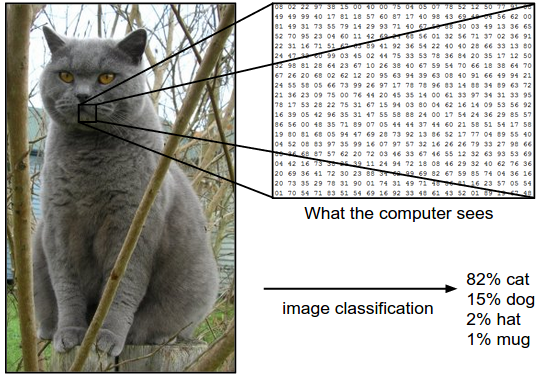
\includegraphics[height=5cm,keepaspectratio=true,clip=true]{imagenes/MarcoTeorico/cv-1.png}
  \caption{Representación de una imagen}
	\label{Fig: cv-1}
\end{figure}


En \ac{cv} tratamos de describir el mundo real que vemos en una o mas imágenes y reconstruir sus propiedades, tal como la forma, iluminación y distribución del color \citep{Szeliski}; con esta disciplina podemos saber en que carril se encuentra un vehículo, cuantas personas hay en una escena, reconocer a una persona en particular. Así como lo mencionado, existen numerosas aplicaciones que hoy en día están en el mercado  y usan técnicas de \ac{cv}. 

Debido a la complejidad de los nuevos desafíos a solucionar las técnicas de \ac{cv} y \ac{ml} se interceptan; de esta manera \ac{cv}  se convirtió en en unos de los dominio principales en los que se han aplicado con éxito métodos de \ac{ml} por ejemplo reconocer objetos en una imagen. 
%https://blogs.zeiss.com/digital/the-relation-between-computer-vision-and-machine-learning/

%\subsection{Ajuste de Modelos}

\subsection{Redes Convolucionales}\label{sub:cnn}
%https://www.researchgate.net/publication/%309455781_Comparacion_de_Arquitecturas_de_Redes_Neuronales_Convolucionales_para_la_Clasificacion_de_Imagenes_de_Ojos
\ac{cnn} son una clase de redes neuronales muy utilizadas en la actualidad por profesionales en \ac{cv}. La arquitectura de una \ac{cnn} consiste en múltiples capas donde cada una de estas tienen diferente propósito.

\begin{figure}[h]
 \centering
  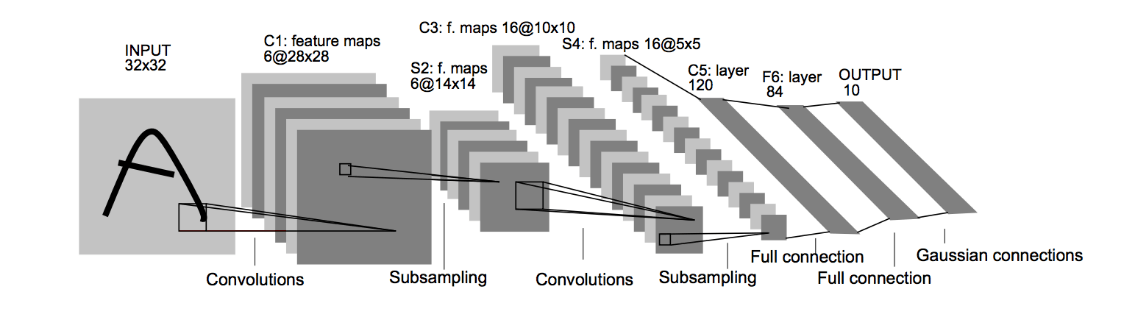
\includegraphics[height=5cm,keepaspectratio=true,clip=true]{imagenes/Logos/cnnconv.png}
  \caption{Red Neuronal Convolucional (Adaptado de:\citep{cnns})}
	\label{Fig: redconvolucion}
\end{figure}

Las \ac{cnn} trabajan modelando de forma consecutiva pequeñas piezas de información (sub-regiones) de la imagen; combinando esta información de salida en las capas mas profundas (ver: \ref{Fig: redconvolucion}), tales características pude ser fusionada pre-procesando con el fin de detectar características de mayor orden \citep{murphy}.


El conjunto de salidas de las neuronas en un plano se denomina \textit{mapa de características} (ver \ref{Fig: fmaps}). Cada unidad  del mapa de característica es lo que llamamos en la sección (\ref{sub:problemadeteccion}),  \textit{\textbf{feature vector}}. Una capa convolucional completa está compuesta de varios mapas de características (con diferentes 
\textit{feature vector}), de modo que se pueden extraer múltiples características en cada ubicación \citep{cnns}.

\begin{figure}[H]
 \centering
  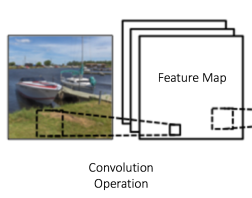
\includegraphics[height=6cm,keepaspectratio=true,clip=true]{imagenes/Logos/fmaps.png}
  \caption{Ejemplo de mapa de características, (Adaptado de: \citep{cnnsarticle})}
	\label{Fig: fmaps}
\end{figure}

El tamaño del mapa de características se controla mediante tres parámetros \citep{cnnsarticle}:
\begin{enumerate}
\item depth (profundidad): corresponde al numero de filtros usados para la operación de convolución. Por ejemplo la primera capa toma la imagen original, luego diferentes neuronas a partir de la profundidad de la red se activa realizando operaciones como puede ser detección de bordes, color, etc
es decir a partir de la imagen de entrada aplicar por ejemplo detección de bordes, color, etc.
\item stride (paso): es el número de píxeles por los que se desliza nuestra matriz de filtro sobre la matriz de entrada. Tener un stride grande producirá mapas de características más pequeños.
\item zero-padding (cero-relleno): A menudo, es conveniente rellenar la matriz de entrada con ceros alrededor del borde, de modo que podamos aplicar el filtro a los elementos fronterizos de nuestra matriz de imagen de entrada. Una buena característica de cero relleno es que nos permite controlar el tamaño de los mapas de características.
\end{enumerate}

Las \ac{cnn} están basadas en operaciones de convolución; la convolución son operaciones de productos y sumas entre las capas y los $n $ filtros (kernel) que generan como se mencionó anteriormente un mapa de característica. La ventaja es que el mismo filtro permite extraer la misma característica en cualquier parte de la entrada, con esto se consigue reducir el número de conexiones y el número de parámetros a entrenar en comparación con una red \textit{fully connected}.

\begin{figure}[h]
 \centering
  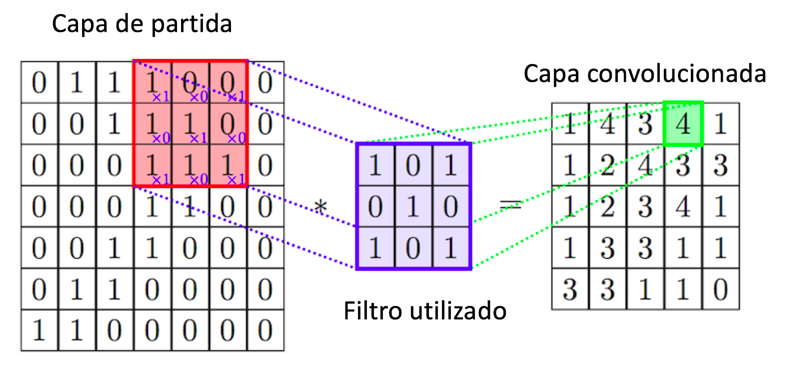
\includegraphics[height=5cm,keepaspectratio=true,clip=true]{imagenes/MarcoTeorico/convolucion.png}
  \caption{Convolución}
	\label{Fig:convolucion}
\end{figure}
%https://www.scribd.com/document/271869018/Convolucion-con-CNN
Las aplicaciones de mayormente utilizadas son: reconocimiento de imágenes, análisis de video, procesamiento de lenguaje natural, detección de poses, segmentación de imágenes, entre otros.
\subsubsection*{Arquitecturas de redes convolucionales}\label{sub:arquitecturacnn}
%https://towardsdatascience.com/neural-network-architectures-156e5bad51ba
La arquitectura de una red neuronal es la forma en que se organizan  las neuronas en su interior, estas neuronas se agrupan formando capas que pueden llegar a tener diferentes características. A continuación desarrollamos las diferentes arquitecturas, topologias, usadas en \ac{cnn}: (extraido de https://towardsdatascience.com/neural-network-architectures-156e5bad51ba)
\begin{itemize}
\item \textbf{LeNet5}: Fue una de las primeras \ac{cnn} que impulso el campo de \ac{dl}, la principal idea de esta red es que determinadas característica se distribuyen sobre toda la imagen; de esta manera convoluciones con los mismos parámetros pueden extraer de manera eficiente esas mismas características en toda la imagen, es decir en múltiples locación. 

LeNet5 esta formada por 3 capas, usando la capa convolucional para extraer las características espaciales de la imagen. En general esta red fue el origen de muchas de las arquitecturas modernas.

\item \textbf{AlexNet}: Esta arquitectura surgió en el 2012 ganadora de la competición \textit{ImageNet}\footnote{http://www.image-net.org/challenges/LSVRC/}. EL problema resuelto en la competición era poder clasificar una imagen dentro de 1000 categorías. Cuenta con 60 millones de parámetros y 650.000 neuronas; AlexNet consta de 5 capas convoluacionales con diferentes kernel que extraen diversas característica de la imagen  y 3 capas \textit{fully connected}. Una importante característica es el uso de \textit{ReLU}(Rectified Linear Unit),  AlexNet demostró que al usar la no linealidad ReLU,  podrían entrenarse mucho más rápido que  funciones de activación como  tanh o sigmoide.

\begin{figure}[H]
 \centering
  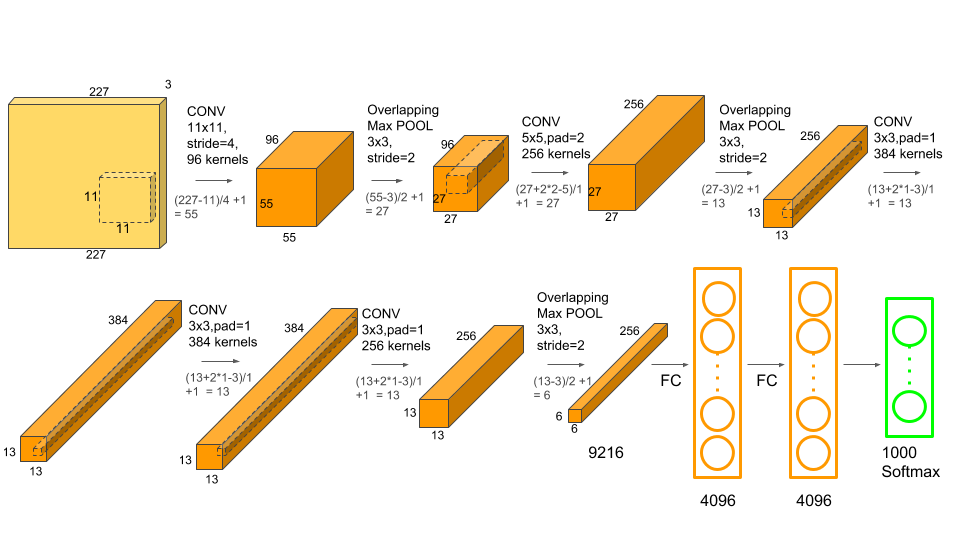
\includegraphics[height=7cm,keepaspectratio=true,clip=true]{imagenes/MarcoTeorico/AlexNet-1.png}
  \caption{Arquitectura AlexNet}
	\label{Fig:alexnet}
\end{figure}


\item \textbf{VGG}: Esta arquitectura se caracteriza por ser la primera en utilizar filtros 3 × 3 mucho más pequeños en cada capa convolucional y ademas los combinaron como una secuencia de convoluciones. La principal contribución de VGG, ganadora de la competición en 2014 de \textit{ImageNet}, es mostrar que la precisión de la clasificación y localización de un objeto en una imagen puede mejorarse al aumentar la profundidad de la \ac{cnn}.

\begin{figure}[H]
 \centering
  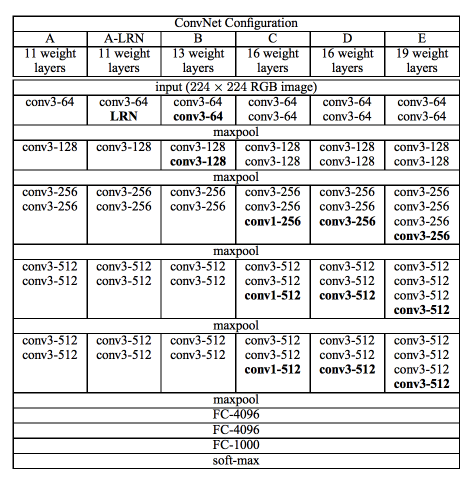
\includegraphics[height=10cm,keepaspectratio=true,clip=true]{imagenes/MarcoTeorico/vgg.png}
  \caption{Arquitectura VGG, (Simonyan and Zisserman (2014)).}
	\label{Fig:vgg}
\end{figure}

\item \textbf{GoogleNet}: EL principal objetivo de esta arquitectura desarrollada es mejorar la utilización de recursos computacionales, esto lo logra definiendo módulos llamados, \textit{módulos inception}, y aumentando la profundidad y el ancho de la red. 
\begin{figure}[H]
 \centering
  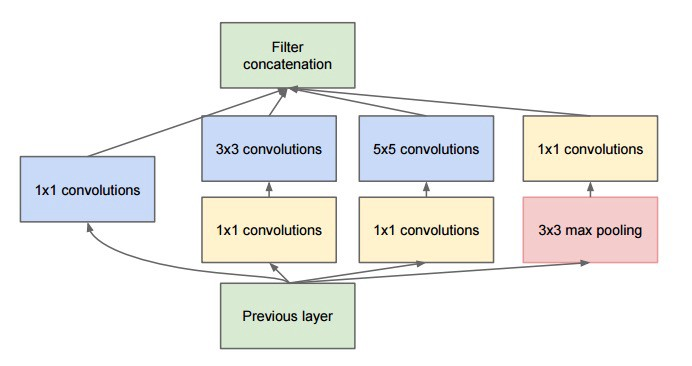
\includegraphics[height=5cm,keepaspectratio=true,clip=true]{imagenes/MarcoTeorico/inception-1.jpg}
  \caption{Arquitectura GoogleNet: modulo inception}
	\label{Fig:inception}
\end{figure}
Como se puede ver en la imagen anterior \ref{Fig:inception} se diseño módulos para luego agruparlos uno arriba de otro. GoogleNet usa un nuevo termino llamado \textit{Bottleneck layer} que permite reducir el numero de características y sus operaciones 

\item \textbf{ResNet}: Es otro tipo de arquitectura nombrada \textit{"Deep Residual Learning"}, a partir de mapeo subyacentes de $x y H (x)$, es posible aprender la diferencia entre los dos, que es el \textit{residuo} y, posteriormente, ajustar el último a la entrada; siendo el residuo $F(x) = H(x) - x$.

\begin{figure}[H]
 \centering
  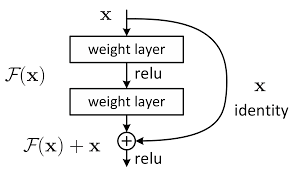
\includegraphics[height=5cm,keepaspectratio=true,clip=true]{imagenes/MarcoTeorico/resnet.png}
  \caption{ResNet:\textit{Residual block}}
	\label{Fig:inception}
\end{figure}

\end{itemize}

En el estado del arte actual existen diferentes variantes que parten de la idea principal de cada arquitectura mencionada anteriormente como: ResNet50, ResNet101, GoogleNet(InceptionV1, InceptionV3), entre otras. En la siguiente figura \ref{Fig:cnn-analisis} se muestra un análisis realizado\footnote{https://arxiv.org/abs/1605.07678} comparando \textit{accuracy} vs \textit{cantidad de operaciones} realizadas en solo una pasada en toda la red.
%https://www.deeplearningitalia.com/guia-para-arquitecturas-de-redes-profundas/

\begin{figure}[H]
 \centering
  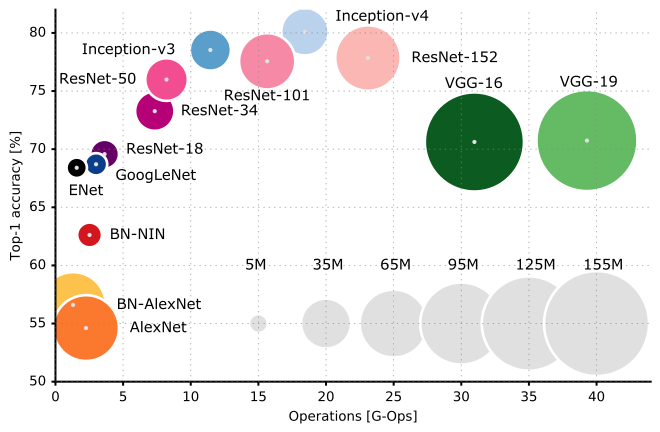
\includegraphics[height=7cm,keepaspectratio=true,clip=true]{imagenes/MarcoTeorico/cnn-analisis.png}
  \caption{ResNet:\textit{Residual block}}
	\label{Fig:cnn-analisis}
\end{figure}

\subsection{Regions Proposal} \label{sub:regions-proposal}

Regiones Propuesta, \ac{rp} en su traducción al ingles, son un conjunto de métodos que permiten extraer regiones dentro de la imagen siguiendo algunas características similares como contorno, color, etc. El proceso metodológico básico es el siguiente: dada una imagen de entrada, este método busca generar un conjunto de regiones candidatas que son localizadas en un \textit{bounding box}, un \textit{bounding box} es la región de interés, que probablemente contengan objetos de interés para la detección (ver: \ref{Fig: propsalregion}), permiten tener ventanas(bounding box) de diferentes escalas. Estos objetos de interés detectados a partir del método son los que posteriormente vamos a clasificar.

\begin{figure}[H]
 \centering
  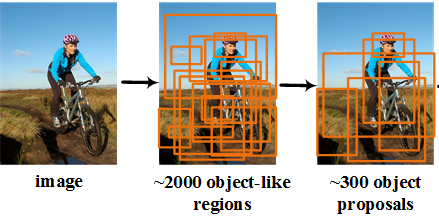
\includegraphics[height=4cm,keepaspectratio=true,clip=true]{imagenes/Logos/regionProposal.png}
  \caption{Ejemplo \ac{rp} \\ (Adaptado de:{http://www.cs.toronto.edu/~byang/})}
	\label{Fig: propsalregion}
\end{figure}

Existen diversos métodos para calcular regiones candidatas que podemos encontrar en: \citep{proposal}. En esta tesis se realizo pruebas con los  los métodos \textit{Edges Boxes} y \textit{Selective Search}.

\subsubsection*{Edges Boxes} \label{sub:edgesboxes}

Edges Boxes es un enfoque para la generación de regiones candidatas a partir de los bordes detectados. Utilizando estructuras de datos eficientes, se pueden evaluar millones de boxes (cajas) candidatos en una fracción de segundo; los bordes proporcionan una representación simplificada pero informativa de una imagen \citep{edges}.

Los algoritmos para la detección de bordes tradicionales utilizan una variedad de métodos para calcular gradientes de color, en el caso de los nuevos enfoques además utilizan múltiples características como entrada; incluyendo brillo, color, textura y  escalas de la imagen. 

En la figura (\ref{Fig: edges}) podemos ver de manera simplificada los pasos del método;  en la parte inferior de la imagen vemos que luego de varios operaciones identifica regiones que podrían ser de interés.

\begin{figure}[H]
 \centering
  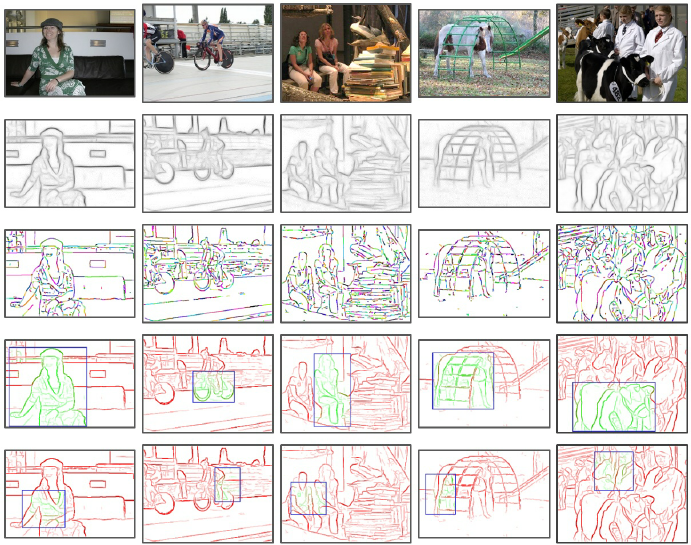
\includegraphics[height=7cm,keepaspectratio=true,clip=true]{imagenes/Logos/edges.png}
  \caption{Ejemplo proceso detección de bordes (Adaptado de:\citep{edges})}
	\label{Fig: edges}
\end{figure}

Este método evalúa las cajas candidatas utilizando un enfoque de ventana deslizante, similar a la detección de objetos tradicionales; donde en cada posición del objeto evaluamos, escala y relación generando una puntuación (score) que indica la probabilidad de que un objeto esté presente en el bounding box.


\subsubsection*{Selective Search} \label{sub:selectivesearch}
Selective Search es un método de \ac{rp} que  permite obtener regiones candidatas realizando una búsqueda exhaustiva aplicando segmentación sobre la imagen. La segmentación  en procesamiento de imágenes consiste en dividirla en grupo de píxeles u objeto. El objetivo es simplificar la representación logrando que sea mas significativa, fácil de analizar y capturar todas las ubicaciones de objetos posibles; en lugar de una sola técnica para generar ubicaciones , diversifica la  búsqueda y usa  una variedad de particiones de imágenes complementarias para tratar con tantas condiciones de imagen como sea posible \citep{selectivesearch}.
Las estrategias usadas en este método son:
\begin{itemize}
\item \textbf{Capturar todas las escalas}: los objetos pueden estar en cualquier escala de la imagen, es por esto que se toma en cuenta todas las escalas.
\item \textbf{Diversificación}: No existe una sola estrategia sino que una región puede formar un objeto solo por color o textura.
\item \textbf{Rápido computo}: Esta es una de las estrategias principales debido a que el objetivo es producir un conjunto de regiones propuesta de manera eficiente y sin un costo computacional alto.
\end{itemize}

\begin{figure}[h]
 \centering
  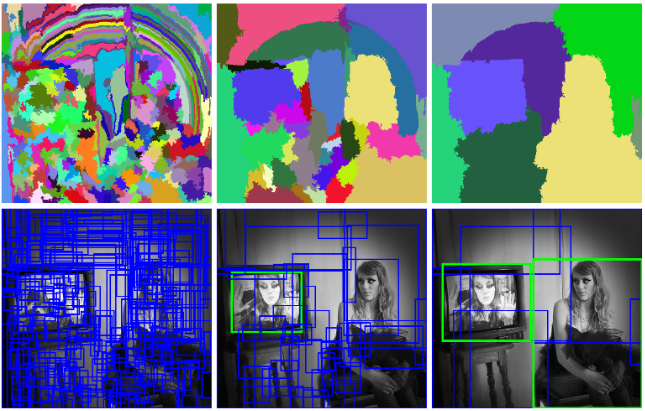
\includegraphics[height=7cm,keepaspectratio=true,clip=true]{imagenes/Logos/selectivesearch.png}
  \caption{Ejemplo segmentación con \textit{Selective Search} (Adaptado de:\citep{selectivesearch})}
	\label{Fig: overlapping}
\end{figure}

\subsection{Non-Maximum Suppression}\label{sub:nonmaximumsuppression}

\ac{nms} es un pre-procesamiento muy importante en el ámbito de \ac{cv}  donde trabajamos con imágenes de alta resolución \citep{nms};  \ac{nms} normalmente se usa con algoritmos de detección de bordes \textit{Edge Boxes}. Puede  suceder que cuando aplicamos métodos de regiones propuestas existan boxes (regiones) con sobremuestreo, es decir lo que en la literatura se los llama \textit{overlapping bounding boxes} , como por ejemplo ver en la figura (\ref{Fig: overlapping}). 

\begin{figure}[H]
 \centering
  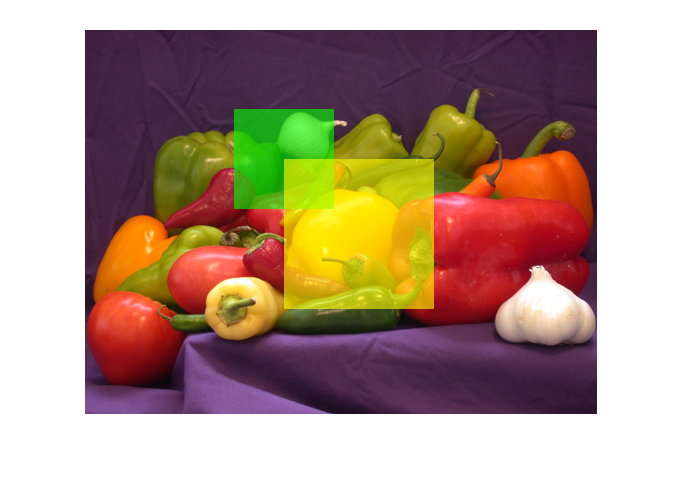
\includegraphics[height=7cm,keepaspectratio=true,clip=true]{imagenes/Logos/overlapMat.png}
  \caption{Overlapping entre regiones (Adaptado de:{https://goo.gl/ihYMvX})}
	\label{Fig: overlapping}
\end{figure}

Para poder eliminar este solapamiento (detecciones redundantes) utilizamos \ac{nms}. \ac{nms} puede ser formulado como una búsqueda de los máximo locales, donde el máximo local es  mayor que todos sus vecinos (\ref{Fig: interseccion}). El algoritmo selecciona aquellas detecciones con un \textit{score} (intersección) alto y elimina los vecinos mas cercanos ya que es muy probable que cubran el mismo objeto \citep{nms2}.

\begin{figure}[h]
 \centering
  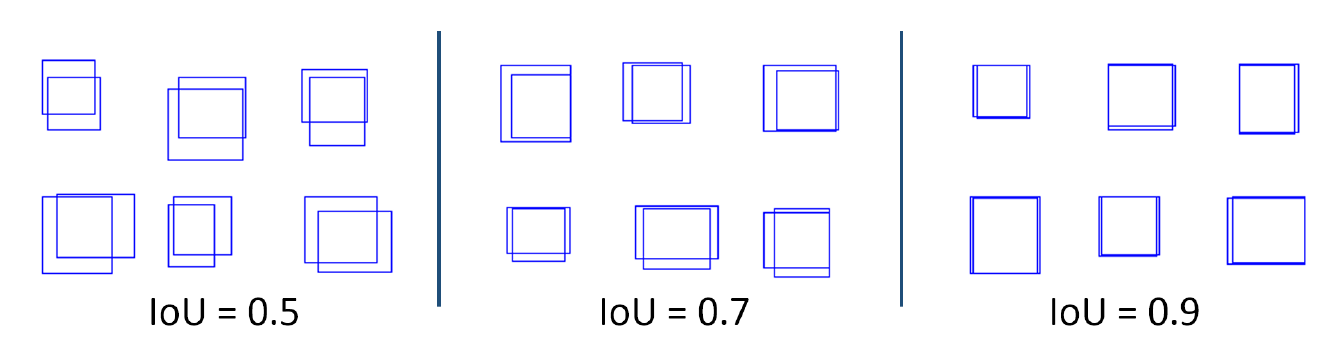
\includegraphics[height=4cm,keepaspectratio=true,clip=true]{imagenes/Logos/overlapping.png}
  \caption{Ejemplo de Overlapping con diferentes scores. (Adaptado de:\citep{edges})}
	\label{Fig: interseccion}
\end{figure}

Dependiendo del valor de score usado podremos eliminar las detecciones redundantes y lograr una mayor optimización  en el reconocimiento. Para obtener una visión mas general del método podemos ver la siguiente figura \ref{Fig: nonmaximumsuppression}.

\begin{figure}[H]
 \centering
  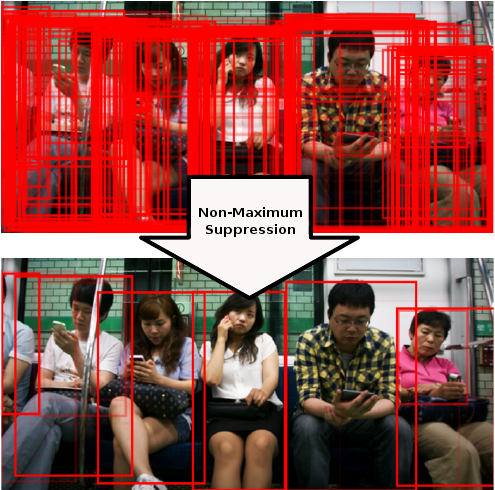
\includegraphics[height=8cm,keepaspectratio=true,clip=true]{imagenes/Logos/nms.png}
  \caption{Uso de non-maximum suppression. (Adaptado de:\citep{nms2})}
	\label{Fig: nonmaximumsuppression}
\end{figure}

En \ac{cv} este método es muy utilizado ya que nos permite además de eliminar detecciones redundantes, ayuda a mejorar la clasificación de la imagen optimizando también el tiempo de procesamiento en la clasificación.


\subsection{Clasificadores}\label{sub:clasificadores}

Un clasificador es un método que permite a partir de recibir cierta información del objeto es capaz de indicar la categoría o clase a a que pertenece determinado objeto. Existen diversos tipos de clasificadores en la actualidad que nombraremos a continuación:

\begin{enumerate}
\item \textbf{Logistic Regression}: son un tipo de clasificadores que permite analizar un conjunto de datos en el cual hay una o más variables independientes. El objetivo de este método es encontrar un mejor modelo que describa la relación entre la respuesta del modelo dado las variables independientes(variables predictivas o explicativas). 

Para asignar los valores predichos a las probabilidades, usamos la función sigmoidea que mapea cualquier valor real en otro valor entre 0 y 1, que tiene la siguiente forma:
\begin{equation}
\phi(z) = \frac{1}{1+e^{-z}}
\end{equation}

\begin{figure}[H]
 \centering
  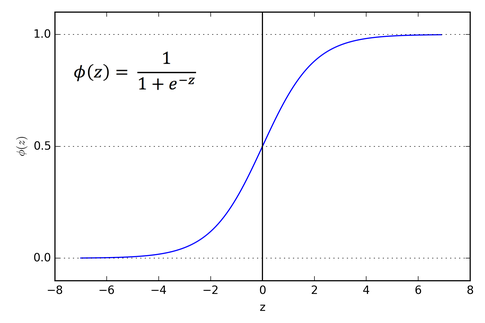
\includegraphics[height=6cm,keepaspectratio=true,clip=true]{imagenes/MarcoTeorico/sigmoide.png}
  \caption{Logistic Regression}
	\label{Fig: log_reg}
\end{figure}


\item \textbf{Decision Tree}: Estos tipos de clasificadores toman un conjunto finito de valores  que toman la forma/estructura de un árbol desglosando el conjunto de datos de entrada en subconjuntos mas pequeños. El resultado final es un árbol con nodos de decisión y nodos de hoja; un nodo de decisión tiene dos o más ramas y un nodo hoja representa una clasificación o decisión. Los árboles de decisión pueden manejar tanto datos categóricos como numéricos.
	
\begin{figure}[H]
 \centering
  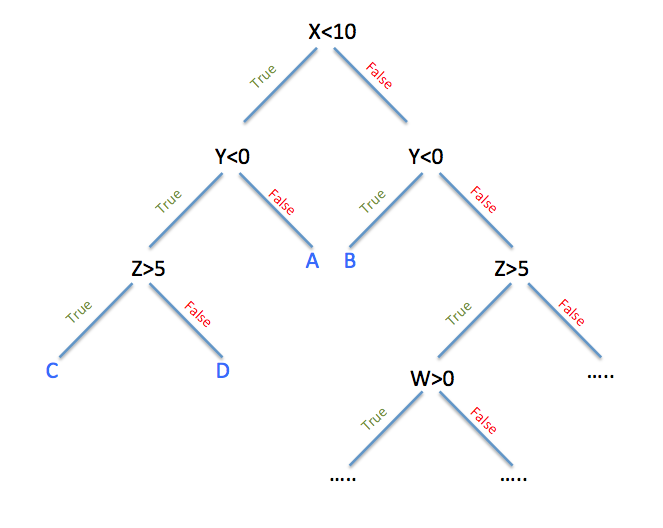
\includegraphics[height=8cm,keepaspectratio=true,clip=true]{imagenes/MarcoTeorico/decision-tree.png}
  \caption{Ejemplo Arboles de desiciones}
	\label{Fig: decision-tree}
\end{figure}


\item \textbf{Random Forest}:Este  algoritmo combina diferentes algoritmos de igual o diferentes tipos para realizar la clasificación; son llamados algoritmos de ensamble. Por ejemplo, ejecutar la predicción sobre \textit{SVM} y \textit{Decision Tree} y luego tomar el voto para la consideración final de la clase del objeto que se esta evaluando. 

\begin{figure}[H]
 \centering
  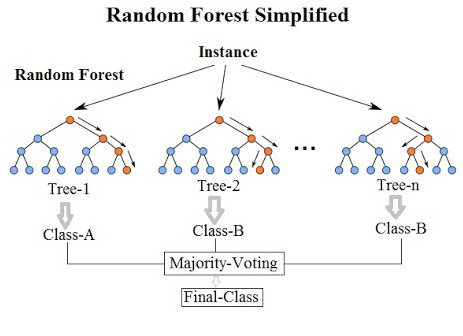
\includegraphics[height=8cm,keepaspectratio=true,clip=true]{imagenes/MarcoTeorico/random-forest.jpg}
  \caption{Ejemplo Random Forest}
	\label{Fig: random_forest}
\end{figure}

\item \textbf{Support Vector Machines, SVM}: Un clasificador SVM busca el limite que separa las clases con el mayor margen posible; como podemos ver en la siguiente imagen (\ref{Fig: margenseparacionsvm}).

\begin{figure}[H]
 \centering
  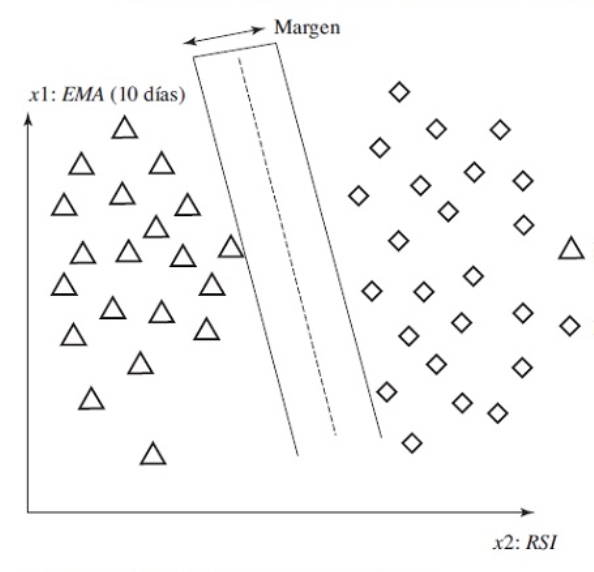
\includegraphics[height=5cm,keepaspectratio=true,clip=true]{imagenes/Logos/separacionsvm.png}
  \caption{Ejemplo margen de Separación hiperplano SVM \\(Adaptado de:{https://goo.gl/eTZfvH})}
	\label{Fig: margenseparacionsvm}
\end{figure}

Las ventajas de estos clasificadores son:
\begin{itemize}
\item Eficaz en grandes espacios dimensionales.
\item Sigue siendo efectivo en casos en los que el número de dimensiones es mayor que el número de muestras.
\item Versátil: se pueden especificar diferentes funciones del kernel para la función de decisión.
\item El proceso de entrenamiento es más rápido en comparación con otros clasificadores, sobre todo para conjunto de entrenamientos grandes.
\end{itemize}

\item \textbf{Nearest Neighbor}: Es otro tipo de clasificador supervisada que busca estimar la probabilidad a posteriori de la clase, es decir,  asigna la muestra $x $ a la clase más frecuente de entre sus $k $ vecinos más cercanos, según una cierta medida de similitud o distancia.

Se calcula la distancia entre los vectores almacenados y el nuevo vector y se seleccionan los $k $ ejemplos más cercanos, una distancia alta entre individuos nos indica que son muy diferentes y una baja que son muy similares. El cálculo de distancia esta dado por la siguiente formula:
\begin{equation}
dist(p,q) = \sqrt{\sum_{i=1}^{n} (p_i - q_i)^{2}}
\end{equation}


Es uno de los clasificadores más utilizados por su simplicidad. La principal dificultad de este método consiste en determinar el valor de $k$.
%http://scielo.sld.cu/scielo.php?script=sci_arttext&pid=S1684-18592016000300008
\end{enumerate}